\chapter{Experiment and Results}

\section{Measurement of Optical Rectification}

We are interested simply in measuring the sign of $d_{eff}$ and
this can be done by measuring the direction of the DC electric
field that is generated within the crystal.  Since optical
rectification is a second order process, a rather large electric
field must be used in order to see some result; it must be
comparable to that used to generate second harmonic fields.  In
our current setup we employ a Q-switched Nd:YAG laser capable of
producing pulses with energies of up to 100 mJ of 10 ns duration
at a wavelength of 532 nm. If we approximate the pulse as a square
pulse in time, then this correlates to a peak power of 10 MW.

The DC electric field is measured by placing parallel conducting
plates perpendicular to the field and then measuring the voltage
that is induced across them.  A diagram of the configuration used
to make this measurement is shown in figure (\ref{ORexp}).

\begin{figure}
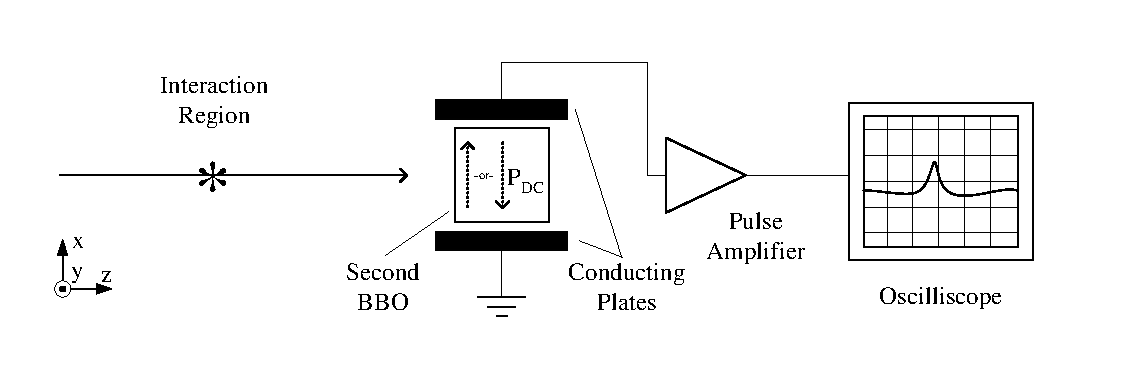
\includegraphics{ORexp}
\caption[Optical rectification measurement apparatus]{Diagram of
the experimental setup used to measure the optical rectification
signal in a BBO crystal}
\label{ORexp}%
\end{figure}

The crystal used in this experiment is a $\beta$-Barium Borate
(BBO) that has an open face of 5mm$\times$4mm and is 5mm in
length. It is oriented for Type I phase matching which means that
the fundamental field and the harmonic field are polarized
perpendicularly to one another.  In this case, the fundamental
field has a polarization along one of the crystal's ordinary axis,
and the second harmonic, as well as the optical rectification
signal, are created along the extraordinary axis. These
orientations are also shown in figure (\ref{ORexp}).

While the short duration pulses from the Nd:YAG laser do allow for
higher peak power, they also make the DC measurement more
difficult since the DC field is essentially only present when the
optical field is driving it.  We therefore need a fast detector
that is capable of detecting the polarity of pulses of 10 ns
duration.

[amplifier/scope configuration]

\section{Choice of Laboratory Coordinate System}

Care must be taken in adhering the laboratory coordinate system.
Since our goal is only to determine the sign of the term
$d_{eff}$, any error in the orientation of the coordinates may
have the result of changing the result to its opposite.  All
calculations and measurements must adhere to these coordinates for
the same reason. These include the phase shift in moving to the
far field, the orientation of the camera imaging system, the
experimental image fitting program, and the orientation of the
phase detection BBO.

Recall, that the coordinate system is defined in the following
way. The positive $z$-axis points in the direction of the beam's
propagation, and the positive $y$-axis is normal to the optical
table.

The first thing that must be accounted for is the orientation of
the camera in the imaging system.  The camera is positioned
looking down on the interaction region, with the optical beam
entering from the top of the image.  Therefore, the collected
image lies in the $x$-$z$ plane with the origin in the upper left corner of the image.  

%positive directions as indicated in figure (\ref{imgcoord}).

%\begin{figure}
%\includegraphics{imgcoord}
%\caption[Image coordinates]{Example experimental image showing the
%orientation of the coordinate system}
%\label{imgcoord}%
%\end{figure}

This experiment uses an algorithm to fit the theoretical equations
to the experimental images.  Since the expected images will be
asymmetric, it is important that the coordinate system used in the
program coincides with that of the image that is passed to it.
Therefore, care must be taken to insure that the orientations of
the spherical harmonics in equation (\ref{angdistsimp}) match
correctly.

Finally, the sign of $d_{eff}$ that is measured will depend on the
choice of coordinate system as well.  Since we are using Type I
phase matching in the second doubling crystal and the incoming
electric field polarization is vertical (in the $z$ direction) we
expect the polarization of the second harmonic as well as the
optical rectification field to be horizontal (in the $x$
direction).  Therefore, we expect

\begin{equation}
P^{(2)}_x = 2d_{eff} \left| E_y \right|^2.
\end{equation}

Determining the sign of $d_{eff}$ now comes to determining if the
DC polarization points in the positive or negative $x$-direction
in our coordinate system.

\section{Determination of Optical Rectification Direction and Optical Phase Shift}





\section{Verification of Independence of Choice of Coordinate System}

Since it appears that the determination of the phase shift depends 
only on the choice of coordinates, some confusion may arise from 
the seemingly abitrary choice of coordinate system.  It appears that
if we measure a polarization in one direction and then choose the
positive $x$-direction to coincide with that, we will end up with a 
$-\frac{\pi}{2}$ phase shift during SHG.  If we were to choose the 
positive $x$-direction to be opposite, then we will end up with a 
$-\frac{\pi}{2}$ phase shift.  The confusion stems from the fact that 
we are trying to determine the phase difference between two waves that
are polarized in planes perpendicular to each other.

Let us consider an example of two waves of the same frequency polarized 
perpendicularly to each other.  This situation is illustrated in figure
(\ref{perppol}).  The reference wave will be the one polarized perpendicularly
to the plane of the page and the positive direction will be up from the
plane of the page.  If we choose the $a$-direction to be positive, then the
two waves will have zero phase difference.  However, if we choose the $a'$-direction
to be positive, then the two waves will have a phase difference of $\pi$.
Since the calculated phase shift during SHG is not the only thing that 
changes with a change in coordinate system we can begin to see that 
if we choose and adhere to a coordinate system properly, confusion in 
the phase can be eliminated.

\begin{figure}
%\includegraphics{}
\caption[Relative phase of perpendicularly polarized waves]{Relative 
phase of perpendicularly polarized waves}
\label{perppol}
\end{figure}


In the end, it must be true that our determination of the phase
shift that occurs during second harmonic generation must be
independent of our choice of coordinate systems.  The result
should stay the same for any choice.  In order to verify this we
will select an alternate coordinate system, and demonstrate that
the final result remains unchanged.  We must therefore track all
points where the change in coordinates will affect the calculated phase of
the beams.

We will start with a single configuration in our current
coordinate system, and then repeat with a different coordinate
system. The physical aspects of each configuration will remain the
same, that is, the collected image and the direction of the
optical rectification signal will not change.  The two situations
are illustrated in figure (\ref{inde}).

\begin{figure}
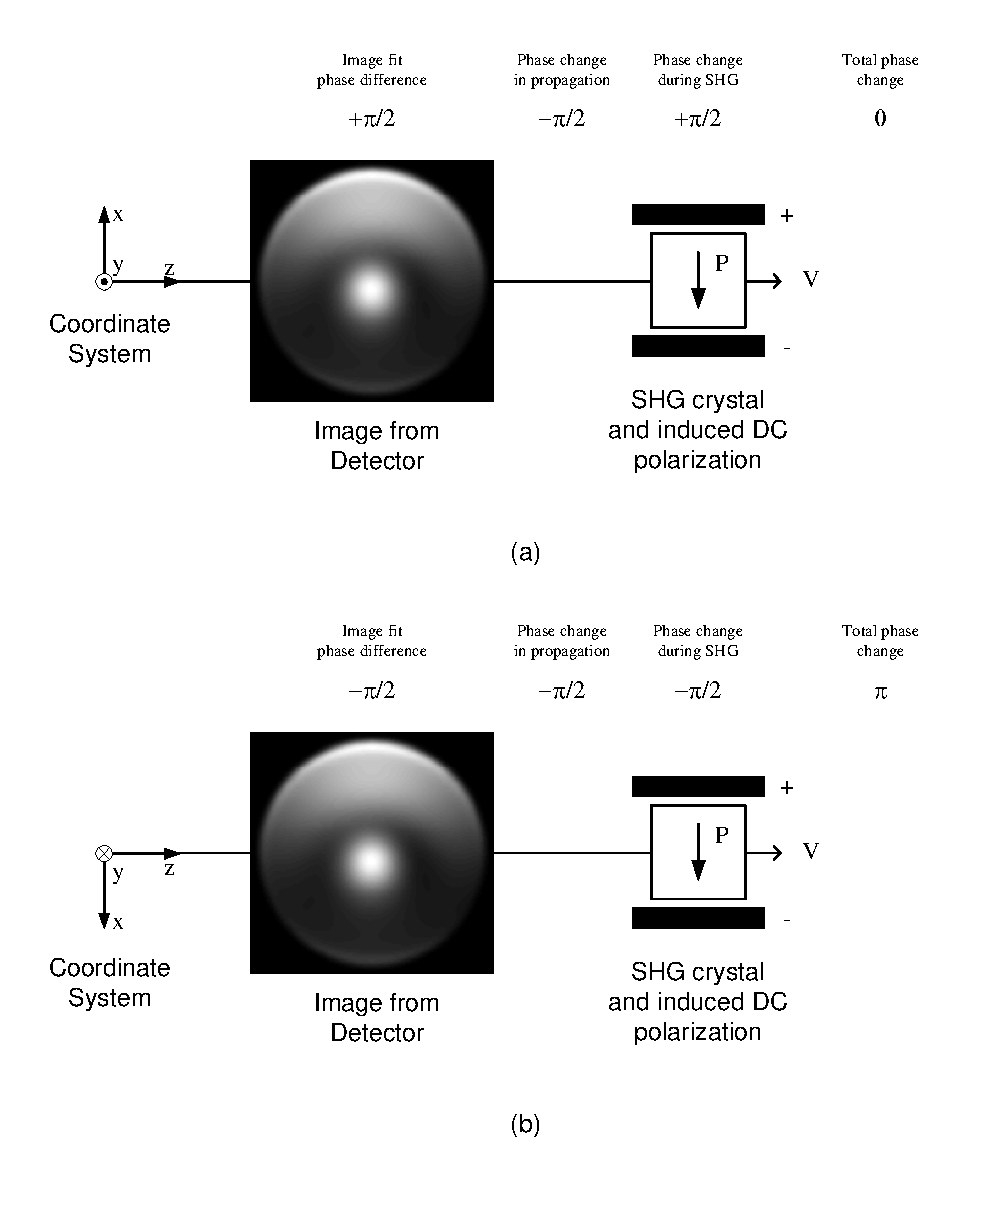
\includegraphics{inde}
\caption[Independence of choice of coordinate system on
result]{Diagram showing quantities that will change with a
corresponding change in coordinate systems. Image (a) represents
the current coordinate system, and image (b) represents an
alternate.}
\label{inde}%
\end{figure}

Let us first examine the situation of the current coordinate
system.  The first thing seen is that the image fitting determines
a phase difference of $+\frac{\pi}{2}$ for the example.  Then, as
determined in section (\ref{phaseshiftff}), there is an additional
phase shift of $-\frac{\pi}{2}$ due to propagation from the focus
into the far field.  Next, since the measured polarization vector
is in the negative $x$ direction as seen in figure (\ref{inde}),
phase shift in second harmonic generation is $+\frac{\pi}{2}$. The
total phase shift sums to zero, which means that the phase
difference as calculated by the image fitting program does not
need to be adjusted, and the phase difference at the interaction
is indeed $+\frac{\pi}{2}$.

For the second coordinate system choice, it is important to make a
note about the behavior of the expected images.  Figure
(\ref{fliptheo}) shows two different experimental images resulting
from two different fields with an optical phase difference of
$\pi$. It can be seen that these are the mirror image of each
other across a line parallel to the $z$ axis.  This means that
reversing the $x$ direction is indistinguishable from changing the
optical phase difference by $\pi$.

\begin{figure}
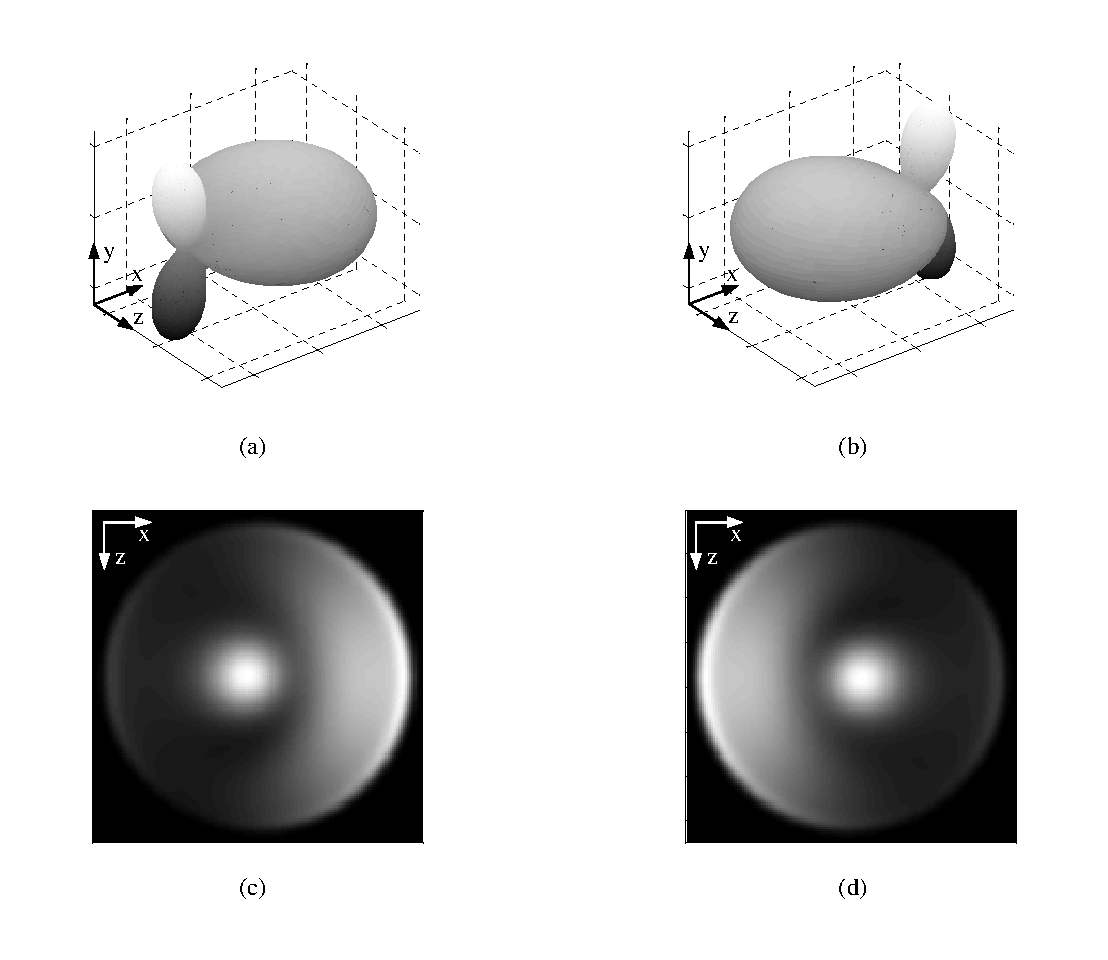
\includegraphics[width=6.25in]{fliptheo}
\caption[Effect of $\pi$ shift in optical phase on detector
images]{Theoretical images demonstrating the differences in images
corresponding to a $\pi$ change in the optical phase.  Image (a)
is the 3D PAD for an optical phase difference of $\pi/2$ and (c)
is the corresponding 2D detector image.  Similarly, (b) and (d)
are the result of an optical phase difference of $-\pi/2$.}
\label{fliptheo}%
\end{figure}

When the image of figure (\ref{inde}(b)) is fit to theory by a
program that has also been modified to account for the change in
coordinate systems, the resulting phase difference will now be
$-\frac{\pi}{2}$ instead of the $+\frac{\pi}{2}$ that was
calculated previously.  The optical fields will experience the
same relative phase change of $-\frac{\pi}{2}$ due to propagation
from the focus.  Looking at the SHG process, the polarization
vector now coincides with the positive $x$ axis, which makes the
phase shift here equal to $-\frac{\pi}{2}$.  This all amounts to a
phase change of $\pi$ that has developed between the fundamental
and second harmonic.  Therefore, the phase measured at the phase
detector is off from the phase at the interaction by a factor of
$\pi$ as well.  If we then adjust the phase calculated by the fit
program by this factor of $\pi$, we ultimately end up with a phase
difference at the interaction of $+\frac{\pi}{2}$.  This matches
with the result from the original coordinate system, showing that
the method of determining the phase shift is indeed consistent.
